\documentclass[a4paper,11pt]{article}


% % % % % % % % % % % % % % % % % % % % % % % % % % % % %
% % ATTENTION : dans les figures le label doit être mis 
%APRES le caption pour que le numéro de la figure lorqu'on
%la référence soit le bon ; sinon on a le numéro du paragraphe
% % % % % % % % % % % % % % % % % % % % % % % % % % % % %

% package qui fournit \justify 
\usepackage[document]{ragged2e}

%pifont pour les puces de formes spéciales
\usepackage{pifont}

% césure exemple
% \hyphenation{an-ti-cons-ti-tu-tion-nel

\usepackage[utf8x]{inputenc}
\usepackage[T1]{fontenc}
\usepackage[frenchb]{babel} % If you write in French
%\usepackage[english]{babel} % If you write in English
\usepackage{lmodern} % Pour changer le pack de police
\renewcommand*\familydefault{\sfdefault}
\usepackage{makeidx}
\usepackage{amsthm}
\usepackage{amsmath}
\usepackage{amssymb}
\usepackage{mathrsfs}
\usepackage{stmaryrd}
\usepackage{geometry}
%\usepackage{graphicx}
\usepackage{graphbox}
\usepackage{supertabular}
\usepackage{tabularx}
\usepackage{longtable}
\usepackage{pdflscape}
\geometry{hmargin=2cm,vmargin=2cm}

\usepackage{booktabs}
\usepackage{tabularx}
\usepackage[table]{xcolor}
\usepackage{ltablex}
\usepackage{float}
\usepackage{url}

\usepackage{chngcntr}
\counterwithin*{footnote}{page}


\usepackage[titletoc,toc,title,page]{appendix}
\renewcommand{\appendixtocname}{Annexes}
\renewcommand{\appendixpagename}{Annexes}

\usepackage{standalone}
\usepackage{ifthen}
\usepackage{xstring}
\usepackage{calc}
\usepackage{pgfopts}
\usepackage{tikz}
\usetikzlibrary{positioning,shapes,shadows,arrows}

\usepackage{algpseudocode}
\usepackage{algorithm}
\makeatletter
\renewcommand{\ALG@name}{Algorithme}
\renewcommand{\listalgorithmname}{Table des algorithmes}

\newtheorem{theo}{Définition}[section]
\usepackage{mathtools, bm}
\usepackage{amssymb, bm}

\usepackage{hyperref}
\hypersetup{
    colorlinks=true,       % false: boxed links; true: colored links
    linkcolor=black,       % color of internal links
    citecolor=purple,       % color of links to bibliography
    urlcolor=blue          % color of external links
}

\usepackage{listings}

\definecolor{dkgreen}{rgb}{0,.6,0}
\definecolor{dkblue}{rgb}{0,0,.6}
\definecolor{dkyellow}{cmyk}{0,0,.8,.3}

\lstset{
  language        = php,
  basicstyle      = \small\ttfamily,
  keywordstyle    = \color{dkblue},
  stringstyle     = \color{red},
  identifierstyle = \color{dkgreen},
  commentstyle    = \color{gray},
  emph            =[1]{php},
  emphstyle       =[1]\color{black},
  emph            =[2]{if,and,or,else},
  emphstyle       =[2]\color{dkyellow}}



\usepackage{blindtext}
\usepackage{enumitem} % pour changer les puces dans \itemize


\date{\today}

\makeindex
\def\siecle#1{\textsc{\romannumeral #1}\textsuperscript{e}}
\newcommand{\argmax}{\mathop{\mathrm{argmax}}\nolimits}
\newcommand{\pgcd}{\mathop{\mathrm{pgcd}}\nolimits}

\makeatletter
\renewcommand{\pod}[1]{\allowbreak\mathchoice
  {\if@display \mkern 18mu\else \mkern 8mu\fi (#1)}
  {\if@display \mkern 18mu\else \mkern 8mu\fi (#1)}
  {\mkern4mu(#1)}
  {\mkern4mu(#1)}
}

\usepackage{wallpaper}

\begin{document}
\renewcommand{\labelitemi}{\textbullet}
% pour factoriser l'échelle des figures 
%utilisation scale=\scaledvwa au lieu de scale = 0.3 ... 
\newcommand{\scaledvwa}{0.4} 
\newcommand{\scaledvw}{0.3}
\newcommand{\scalekad}{0.45}


\phantomsection
\begin{titlepage}
	\parindent=0pt
\ThisTileWallPaper{1.3\paperwidth}{1.0\paperheight}{images/ctrl2}
 
\addtolength{\wpXoffset}{-4.5cm}

%	\vspace*{\stretch{1}}
%	\begin{center}
%		
\includegraphics[scale=0.5]{images/enac.png}%
%	\end{center}
	
\color{white}{	\vspace*{\stretch{1}} }
	\hrulefill
	\begin{center}\bfseries\Huge
		\color{white}
		{Méthodes formelles de conception : Système de contrôle de traffic aéroportuaire} 
	\end{center}
	\hrulefill
	
	\vspace*{1cm}
	\begin{center}\bfseries\Large
			\color{white}
		{Jules Heller - Abdelkader Beldjilali}
		
	\end{center}
	
	\vspace*{\stretch{2}}


\end{titlepage}%on créé la couverture

\pagebreak

\tableofcontents
\justify

\pagebreak

\section*{Introduction}
\addcontentsline{toc}{section}{Introduction}

L'exercice proposé a pour finalité la modélisation et l'analyse d'un système ATC simplifié dans un cadre MBSE. Cette approche permet, en effet, des vérifications précoces intervenant lors de la phase décroissante du cycle en V, juste avant l'implémentation.  

Les composants internes, constitutifs du système ATC considéré, comptent des acteurs humains, les contrôleurs, et des acteurs systèmes hardware et software. On citera les radars primaires, secondaires, les logiciels de traitement, de transport et d'affichage des données radar et plan de vol sans oublier les filets de sauvegarde. Le NMOC européen, Network Management Operation Centre, et le système de traitement de plan de vol national sont inclus dans le système étudié car ils participent à la fourniture du service de contrôle. Par contre, les composants humains, matériels et logiciel associés à l'aspect technique assurant notamment la maintenance des composants ne sont pas pris en compte dans le cadre de cet exercice.

Quant aux acteurs extérieurs, ce sont en particulier les pilotes, les compagnies aériennes, la référence horaire GPS, les aéronefs équipés de transpondeurs, le service météo. On pourrait ajouter les acteurs humains impactant la sûreté et la sécurité du système directement par le hacking du réseau ATC ou par brouillage des communications radio, par détournement de vols, etc. Ceci impacte sur les contraintes que subit le système sans oublier l'acteur environnemental des phénomènes météo. On choisit cependant de les ignorer également pour se focaliser sur l'objectif pédagogique principal de cet exercice. 









\section{Analyse de marché suivant le modèle de Porter}

\subsection{Concurrence entre les firmes existantes}

\subsubsection{Définition du marché}

Le marché concerne le fret aérien qui désignera dans la suite tous les biens y compris le fret postal à l’exception des bagages. (IATA)

Cette étude porte sur les sociétés de Fret Aérien Civil Traditionnelles (FACT) qui gèrent leur propre flotte aérienne pour le transport de biens. Ce qui exclut le fret militaire ainsi que les logisticiens, entreprises de fret "virtuelles", qui font souvent du point à point par le biais de location de charters ou d'achat d'emplacements aux compagnies de fret traditionnelles. Les compagnies virtuelles constituent donc à la fois des clients pour les acteurs de Fret Aérien Civil Traditionnel (FACT) en leur permettant d'optimiser le remplissage de leurs avions-cargo, mais aussi une forme de concurrence puisque le fret transporté au nom du logisticien est "perdu" pour tous les transporteurs classiques, y compris celui qui assure réellement le service.



\subsubsection{Description des produits concernés}
\label{produits}
Pour évaluer la concurrence, il convient d'étudier en premier lieu le type de produits transportés. En effet, le pétrole ou le gaz, ne sont pas en général, transportés par avions ; sur ces matières premières, le fret aérien ne concurrence pas les secteurs maritimes, routiers, ferroviaires, fluviaux ou par oléoduc/gazoduc. 

Le fret aérien, pour être compétitif, concerne donc les produits à haut rapport valeur-poids, souvent aussi à forte valeur ajoutée, ou à forte contrainte temporelle :


\begin{itemize}
	\item Électronique,
	\item Produits périssables : fleurs, fruits...
	\item Produits urgents (colis express...) ou à finalités humanitaires.
\end{itemize}



\subsubsection{Taxonomie des acteurs du transport du fret}
\label{taxonomie}
On distingue 3 types de sociétés de transport qui exhibent des structures de coûts, des caractéristiques opérationnelles et une répartition spatiale de l'offre et de la demande distinctes.\\


Les \textbf{compagnies de cargo} qui ont pour cœur de métier le seul transport aérien de fret, principalement sur les liaisons long-courriers ou transatlantiques. Ces compagnies possèdent une flotte d'avions tout-cargo dédiés, qui vont du gros porteur B747-8F de rayon d'action 8000 km et de capacité 140 tonnes, au Beluga – Airbus A300 reconverti – jusqu'au simple twin turboprop Cessna super cargomaster (RA : 1700 km, capacité de fret : 1.8 tonnes). Un transporteur de fret classique comme Cargolux a très peu de frais de personnel et de frais commerciaux. En revanche, les coûts liés aux avions, aux redevances aéronautiques et aux frais d’escale sont élevés. Seuls 10 à 15 \% du trafic mondial de fret aérien est réalisé par ce type de compagnies. \cite{popescu}\\
	
Les \textbf{compagnies mixtes} telles que Lufthansa, Air France-KML ou encore Emirates et Korean Air utiliseront soit le transport en soute dans leurs avions-passagers, soit des avions cargo combinés, i.e. des avions configurés de manière permanente pour le transport de fret et de PAX ou des avions reconfigurables rapidement pour les deux types de transport. Pour illustrer le transport en soute, on note qu'un moyen-courrier assurant un vol avec 200 passagers représente un revenu d’environ US\$100 000, auxquels s’ajouteront quelque US\$13 000 en fonction du taux de remplissage des soutes de l’avion. Un moyen-courrier de la catégorie A330/B767 permet d’embarquer environ 10 tonnes de fret hors bagages. En 2015, la valeur moyenne de chaque kilo transporté par avion s’établit à US\$127, contre US\$1,10 pour le maritime.
Certaines compagnies mixtes possèdent aussi des filiales spécialisées dans le cargo. On peut citer par exemple Emirates SkyCargo, classée 3e en terme de fret tonne-kilomètres (FTK) ou British Airways World Cargo classée 12e. Mais même dans ce contexte, British Airways va cesser l'exploitation de ses Boeing 747-8F dédiés pour se recentrer sur les opportunités qu'offre le cargo en soute. \cite{theEconomist01}\\

Les \textbf{intégrateurs}\label{integrateurs} comme FedEx, UPS, TNT ou DHL, qui font du point à point avec des avions tout-cargo via des hubs dédiés, sont des entreprises avec des frais de personnel plus élevés et des coûts avion moindres grâce à une flotte d'appareils d’occasion convertis en cargo : A300-600, A310. \cite{lantenne} Dans leur logique du dernier kilomètre, ces intégrateurs opèrent une chaîne logistique multimodale complète en disposant également de leurs propres entrepôts, camions et maillages routiers.\\

On remarque que le transport de fret en soute peut être facturé au coût marginal car les coûts directs d'exploitation du vol sont imputés aux passagers, ce qui lui offre un avantage concurrentiel sur le tout-cargo. Trois solutions possibles à ce problème : la régulation des prix pour protéger les tout-cargo, le ré-ajustement de la flotte pour les compagnies mixtes qui revendent leur cargo, voire constituent des filiales disjointes, ou la différentiation en offrant des services spécifiques. Ce dernier point vaut notamment pour les entreprises tout-cargo qui ne sont pas astreintes à opérer sur des aéroports destinés au trafic passager ; il s'agit ici de tirer partie
de la souplesse dans la localisation et la topologie du réseau mondial de hubs de fret. Dans ce sens, nous verrons que les intégrateurs ont su s'imposer sur le marché en apportant une solution clé en main.


Enfin, les compagnies mixtes sont soumises à une barrière de sortie du secteur du fret beaucoup plus souple et rentable. Les tout-cargo, quant à elles, n'ont d'autres choix que le rachat par un concurrent ou nouvel entrant, de mettre la clé sous la porte, d'évoluer ou de fusionner. À l'instar du transport de passagers, des alliances permettent des économies d'échelles et des synergies bénéfiques en terme de qualité et versatilité des services proposés au clients. Des ententes illégales sur le prix du fret ont été révélées il y a quelques années, entre Qantas Airways et plusieurs autres compagnies ou encore Air France-KLM, Cathay Pacific et SAS Cargo...\cite{popescu}


\subsubsection{Description du marché}
Le fret aérien génère un chiffre d’affaires annuel évalué par l’Association internationale du transport aérien (IATA) à 47,8 milliards de dollars en 2016. Les avions ont embarqué 53,9 millions de tonnes de fret en 2016. L’aérien ne représente qu’un faible pourcentage du volume du fret (environ 5 \%),
mais environ 35 à 40 \% en valeur. \cite{lantenne}. Ce secteur demeure toutefois une activité minoritaire au sein des compagnies aériennes, le transport de passagers produisant 80 à 85 \% de ses recettes. Le transport maritime constitue le principal concurrent de l’aérien. Du fait de son coût très faible, les entreprises optimisent leur logistique pour rendre compatibles les délais de transport avec leur activité. Les autres modes de fret, a contrario, se présentent parfois comme complémentaires de l'aérien : fret camionné de Toulouse au hub de Roissy-CDG par exemple.

En terme de taille de marché, on comptait en 2015 environ 200 firmes spécialisées dans le cargo, y compris les intégrateurs définis § \ref{taxonomie}, auquel s'ajoute un nombre approximatif de 1100 compagnies aériennes dédiées au transport de passagers et appelées de plus en plus à alimenter l'offre en fret AFTK (Available Fret Tonne-Km) ; les \textit{wide-body} aux capacités en soute augmentée n'y sont pas étrangers.

En 2014, la part de marché en valeur, en revenu tonne kilomètre global (RTK), pour le tout-cargo (compagnies de cargo et intégrateurs) se monte à 56 \%. La tendance depuis 2000 est à la baisse au profit des compagnies mixtes avec transport en soute, avec probablement une part de marché en quantité qui ne dépasse pas désormais les 30 \%. L'adverbe \textit{probablement} souligne ici la difficulté d'obtention et d'interprétation des données aéronautiques. Le tout-cargo est en outre confronté au problème de la \textit{bi-directionnalité} c'est-à-dire au retour à vide après livraison, spécificité qui n'existe pas dans le transport de passagers, et que seules des optimisations en termes de flux et de placement des hubs permettent de soulager.

Pour donner une idée de la répartition des acteurs sur le marché, à défaut de pouvoir obtenir des données plus précises, on remarque en 2014 la prédominance des intégrateurs FedEx (7 millions de tonnes transportés) et UPS (4 Mt) et des compagnies asiatiques et du Moyen-Orient, hub des pays du Golfe : Emirates, Korean Air, Cathay Pacific Airways à Hong-Kong. \cite{top50}

L'évolution du marché est caractérisée par une croissance molle au niveau global et un contraste géographique marqué dû notamment aux hubs du Moyen-Orient et d'Asie. Sans développer davantage, on peut noter que la croissances du fret et du trafic passagers dans ces régions induit un accroissement du surplus de l'offre en fret (AFTK). Chaque mise en service d'un Boeing 777 ajoute 25 tonnes de fret 
à l'offre déjà surdimensionnée grevant ainsi la santé globale du secteur. \cite{theEconomist01}


Au niveau stratégique, le secteur est confronté à divers facteurs : sécurité, environnement, politiques protectionnistes, accords internationaux... L'accord de Bali (décembre 2013) visant à libéraliser les échanges commerciaux en réduisant la bureaucratie aux frontières et en aidant les pays les moins avancés pourrait par exemple multiplier le volume de fret aérien d'un facteur de 1.4 grâce à une baisse généralisée des coûts. \cite{iata.org01} On citera pour finir l'importance
de l'évolution de l'offre aéroportuaire pour éviter les problèmes de congestion.
Le climat peut en être une cause avec un nombre croissant d'aéroports inondables : 40 en Europe, 20 rien qu'en Norvège.
\subsection{Clients}

La nature des clients dépend fortement du type de modèle.

Les intégrateurs s'adressent directement aux entreprises ou aux individus, lesquels attachent une importance particulière à la logistique simplifiée porte-à-porte et aux délais de livraison garantis par une offre multimodale riche. Par ailleurs, les principaux intégrateurs ne se limitent pas au transport aérien et peuvent espérer tirer profit d'autres activités et toucher une clientèle élargie et fidélisée pour laquelle le transport aérien n'est plus une fin.

Les clients directs des compagnies de cargo ou des compagnies mixtes seront des logisticiens qui disposent des infrastructures et équipements nécessaires à la manutention du fret. Le surplus dans l'offre en capacité de fret conduit à une situation où le client
possède un fort pouvoir de négociation : non captif, le client peut changer facilement de fournisseur de service de fret aérien. Ainsi, les compagnies de fret n'ont parfois d'autre choix que de brader leurs prix.

En terme de taille de marché, les États-Unis en 2016 arrivent en tête avec 7.7 millions de tonnes de fret, suivis par l'Allemagne (4.4 Mt), la Chine (3.4 Mt) et Hong-Kong (3.2 Mt), de source IATA.


\subsection{Fournisseurs}

Comme pour toutes les compagnies aériennes, la volatilité et le niveau des prix du pétrole est un souci permanent, compensable cependant par des investissements financiers et les solutions alternatives, réacteur à gaz ou à biocarburant, qui ne sont encore qu'à l'état de prototypes. Les contraintes réglementaires et environnementales imposent également de renouveler les flottes avec des avions plus récents.

Au niveau des constructeurs d'avions, les entreprises de fret sont, peu ou prou, confrontées au duopole Boeing - Airbus. Elles possèdent malgré tout d'une part un pouvoir de négociation proportionnel à leur taille et d'autre part la possibilité de se fournir sur le marché de l'occasion ou de faire appel à la location.

Le secteur du fret est un consommateur captif vis-à-vis des fournisseurs de services aéroportuaires. Les contraintes de volume et de poids imposent des équipements spécifiques permettant de garantir une manutention sûre et efficace, aussi bien pour les phases de (dé)chargement que par l'utilisation d'enceintes à rayons X adaptées. Les sociétés de fret sont aussi dépendantes des créneaux qui lui sont attribués et doivent faire face à la congestion du trafic en travaillant avec les différents acteurs aéroportuaires et de l'ATM. Ceux-ci peuvent alors être perçus comme des compléments auxquels il est difficile de s'abstraire totalement, bien qu'il soit possible dans un premier temps d'opérer tout ou partie d'une plate-forme aéroportuaire dédiée au fret.

Enfin, les compagnies de cargo doivent, pour rester attractives face aux compagnies mixtes et aux intégrateurs, contracter des accords avec des logisticiens pour proposer des services annexes tels que le transfert routier.
\subsection{Menaces d'éventuels entrants}

Pour les intégrateurs, les barrières à l'entrée semblent davantage relever de la présence de mastodontes tels que FedEx, UPS, TNT ou DHL capables de pratiquer des prix bas dûs aux économies d'échelles et disposant d'une forte intégration internationale et locale avec des hubs et maillages routiers optimisés. 


En outre, si la possibilité de louer ses avions plutôt que de les acheter permet de créer des compagnies ariennes fussent-elles éphémères, la sur-capacité actuelle de l'offre favorise plutôt la sortie que l'entrée. Si la demande est destinée à augmenter, la capacité l'est également avec le nombre croissant de \textit{wide-body} en circulation. Les compagnies souhaitant expérimenter le modèle mixte devront ainsi justifier d'un solide réseau de routes et de hubs, ce qui explique aujourd'hui la prépondérance des majors dans ce marché.  

A priori, les nouveaux entrants éventuels se porteront plutôt sur des marchés de niche, à moins qu'ils ne surfent sur l'apport de nouvelles technologies telles que les drones, les avions sans pilotes, le tout numérique pour réduire le coût des formalités et les accélérer, le centraliser. Mais alors les firmes en place ne sont-elles pas les mieux placées pour tirer partie de ces avancées quitte à racheter ces start-up ?
\subsection{Menaces liées à l'existence de substituts}
\label{substituts}

Par son coût élevé, le transport de fret aérien se justifie dans le cadre de certains produits typiques définis au § \ref{produits} pour lesquels il n'existe généralement pas de substituts satisfaisants.

Cependant, dans certains cas, l'optimisation et l'anticipation logistique des entreprises peuvent leur permettre d'être moins dépendantes du transport aérien. Avec des progrès techniques, en termes de conservation et de chaîne du froid par exemple, le transport maritime peut aussi parfois devenir une option viable. Le transport ferroviaire, que l'on estime 80 \% moins cher que le transport aérien, continue lui aussi de se développer notamment entre l'Europe et l'Asie, concurrençant sérieusement le transport maritime et grignotant peut-être demain le marché du fret aérien. \cite{lemonde_train}

Enfin, l'augmentation des coûts de production à l'étranger, le développement du protectionnisme avec les crises, les problématiques liées au respect de la propriété intellectuelle peuvent constituer autant de raisons pour les entreprise de relocaliser leur production. En ce sens, le transport terrestre redevient un concurrent sérieux. 

\section{Aspect fonctionnelle}
	
	\subsection{Décomposition fonctionnelle}
	
	L'analyse du sujet a conduit à quatre fonctions principales décomposées en sous-fonctions selon le diagramme hiérarchique de la figure \ref{hier} :
	
	\begin{itemize}
		\item Acquérir les informations, 
		\item Traiter les informations,
		\item Afficher les informations,
		\item Communiquer
	\end{itemize}

L'analyse du modèle a mis en évidence, s'il était besoin, le rôle crucial
de la communication entre contrôleur et pilote dans la fourniture du service de contrôle, d'alerte et de surveillance. Sur le plan métier, la radio comme moyen de communication constitue le maillon faible des systèmes ATC actuel. En ce sens, la modélisation permet 
de mettre en évidence des failles du domaine réel ce qui constitue une source de progrès. 
	
	\begin{figure}[H]
		\begin{center}	
			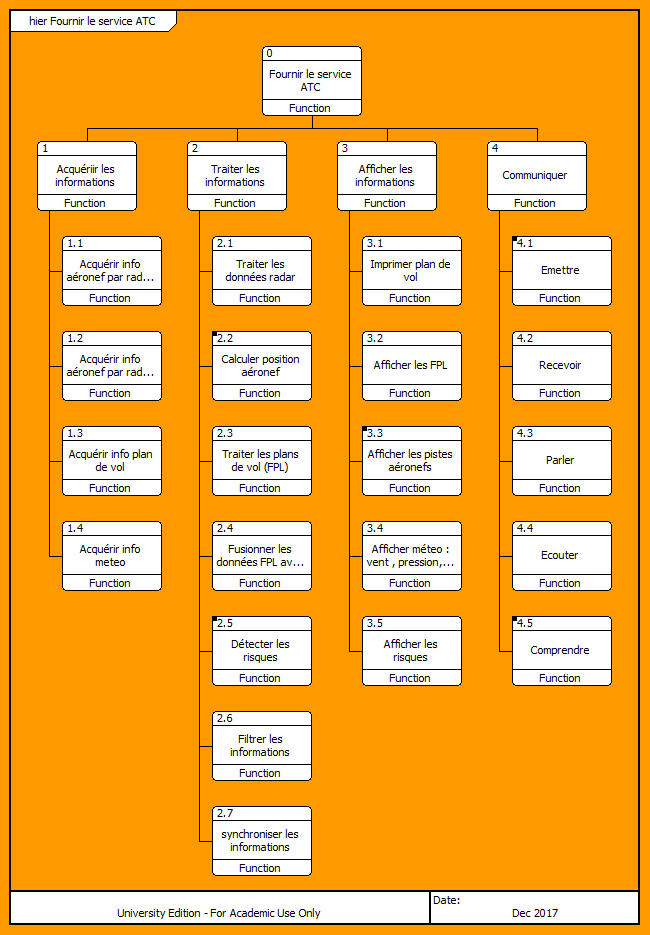
\includegraphics[scale=0.85]{images/hierarchique}
			\caption{Diagramme hiérarchique des fonctions}
			\label{hier}
		\end{center}
	\end{figure}
	
	\subsection{Scénario fonctionnel}

    Les diagrammes d'activités, EFFBD ou de séquence permettent de capturer un ou plusieurs scenarii du système modélisé. La démarche utilisée a consisté à créé un diagramme EFFBD dans CORE en utilisant uniquement les fonctions feuille puis de travailler sur le diagramme N2 pour l'ajout des items. Un exemple est donné en figure \ref{atc}. Le scénario associé à l'ensemble des fonctions feuille se trouve à l'adresse  \url{https://github.com/kad15/AF/blob/master/LIVRABLES_ATC_YUAN_BELDJILALI/question%207%20%20scenario%20fonctionnel%20unique.png}
    
    	\begin{figure}[H]
    	\begin{center}	
    		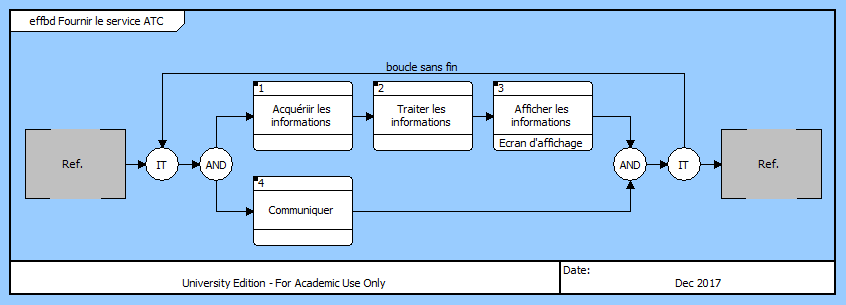
\includegraphics[scale=0.75]{images/atc}
    		\caption{Diagramme EFFBD simplifié du service ATC}
    		\label{atc}
    	\end{center}
    \end{figure}
    

\section{Rôle de l'ATM dans le futur par rapport aux stratégies des acteurs }

L'\textit{Air Traffic Management} est un domaine en perpétuelle évolution, tout particulièrement ces dernières années en Europe. En effet, il s'agit d'un secteur où les procédures et les outils doivent évoluer et s'adapter au trafic afin d'assurer une meilleure gestion du trafic tout en gardant un niveau de sécurité élevé. Nous allons voir un certain nombre d'évolutions qui pourraient avoir un impact sur les acteurs du fret aérien.

\subsection{L'opportunité du programme SESAR}

Comme le montre \cite{52008DC0750}, le programme \textit{Single European Sky ATM Research} (SESAR) mis en place par la Commission Européenne affiche d'ambitieux objectifs tels que :
\begin{itemize}
\item une réduction de moitié des coûts de contrôle aérien;
\item une réduction de 10\% de l'impact sur l'environnement;
\item une division du risque d'accident par 10;
\item un triplement de la capacité de l'espace aérien.
\end{itemize}

Dans ce contexte, les entreprises de fret aérien, au même titre que l'ensemble des compagnies aériennes volant en Europe, vont voir apparaitre la possibilité d'augmenter leurs capacités et de diminuer leurs coûts. Ainsi, si les échanges commerciaux continuent à croitre, notamment avec l'Asie, ces entreprises de transport pourront se développer sans contraintes immédiates dues à la gestion du trafic aérien.

Ces objectifs pourront être rendus possibles par le progrès technique (moteurs plus économiques et moins bruyants), la généralisation de procédures efficaces (descente continue) et la refonte du ciel européen qui souffre aujourd'hui d'une coûteuse segmentation et d'un manque d'harmonisation et de standardisation.\\

On voit donc en quoi les travaux actuels de modernisation de l'ATM permettent d'ouvrir un certain nombre de perspectives aux entreprises de transport aérien en général et, par conséquent, aux entreprises de transport aérien de fret en particulier.

\subsection{Introduction de nouveaux paradigmes}

Dans le cadre des réflexions relatives à la privatisation de certains ANSP (\textit{Air Navigation Service Provider}), des idées de services commerciaux que pourraient vendre ces entités ont émergé.

Par exemple, il serait envisageable de moduler le tarif de la redevance de contrôle en fonction du gain de temps ou du retard que serait prête à accepter une compagnie. Ainsi, une compagnie qui souhaiterait être prioritaire sur l'attribution d'un créneau paierait une redevance plus élevée qu'une compagnie prête à accepter un retard.

Or nous avons pu voir que l'une des spécificités du transport aérien de fret est que les marchandises sont, dans le cas général, résilientes face aux retards. Ainsi, grâce à ces services commerciaux liés à la gestion du trafic, les transporteurs aériens de fret pourraient optimiser leurs coûts dans certains cas.\\

On voit donc que de nouveaux paradigmes émergent au sein des ANSP et que ceux-ci peuvent impacter fortement la stratégie des transporteurs aérien de fret.

\subsection{Vers une extension du périmètre du fret}

%Etablissement de régulation lors du développement des drônes et avions sans pilotes : voilure mobile ou fixe. 

Comme le montre \cite{RePEc:eee:jaitra:v:61:y:2017:i:c:p:34-40}, de nouvelles entrées, certes limitées mais réelles, font leur apparition sur le marché du transport aérien de fret. Il s'agit principalement d'opérateurs de drones souhaitant réaliser un transport de marchandise par le biais de cette nouvelle technologie.

On peut citer notamment des entreprises comme La Poste \cite{gradt_2016} ou Amazon \cite{figaro_2016} qui tentent de mettre en place ce nouveau marché.

Si ce nouveau segment répond plutôt à la problématique du dernier kilomètre qui ne concerne pas tous les acteurs du transport aérien de fret, il est à noter que les évolutions de l'ATM vont jouer un rôle essentiel dans le développement de ce marché.

En effet, l'automatisation du transport aérien de marchandise pose un grand nombre de difficultés au regard de la gestion du trafic aérien dans certains espaces. De nouveaux concepts émergent alors : on parle ainsi de l'UTM (\textit{Unmanned Aircraft Systems} (UAS) \textit{Traffic Management}) au lieu de l'ATM pour désigner ces problématiques de gestion de trafic propres aux drones.\\ 

Ainsi, les évolutions technologiques dans les domaines de l'ATM, de l'UTM et des drones apporteront de nouvelles possibilités de développement aux acteurs du transport aérien de marchandises.






\section*{Conclusion}
\addcontentsline{toc}{section}{Conclusion}


\paragraph{}
La démarche employée est itérative. Dans l'approche MBSE, on divise le système en fonctions et sous fonctions que l'on confrontent d'un côté aux exigences si ces dernières ont été saisie dans CORE et de l'autre aux composants qui assurent ces fonctions. Le tracé de diagrammes dynamiques comme les EFFBD aident à visualiser le système en action et donc à découvrir des fonctions qu'on auraient pu oublier et à régler le niveau de granuralité optimal au même titre que le reporting permis par CORE qui confronte fonctions, composant, item, link.  

\paragraph{}
Le reporting de CORE est aussi une aide précieuse pour la validation du projet en amont par le client et l'évaluation financière et ressources nécessaires à ce dernier.

\paragraph{}
Par manque de temps, les aspects link et requirement n'ont pu être traités. Mais, ils n'étaient pas explicitement demandés. Il manque de plus à ce projet encore de nombreuses itérations ; la précipitation est génératrice de bugs. Enfin, l'aspect maintien en conditions opérationnelles du système ATC n'a pas été abordé, celui du développement de ces systèmes non plus.

\paragraph{}
CORE semble donc aider à construire "the right system and the system right". En particulier permet d'assurer
l'exhaustivité de la prise en compte des exigences par les fonctions. Encore faut-il que les exigences traduisent correctement les besoins.


%\newpage
%\appendix
%\section{Annexe}
\label{annexe_A}

\begin{itemize}
\item Pour écrire simplement les clés sur le disque, nous utilisons Marshal, qui garantit la compatibilité entre toutes les plateformes pour une même version de OCaml.
\item Bien que BatIO propose une API pour manipuler les canaux au niveau du bit, nous avons préféré rester au niveau de l'octet car il s'agit d'une solution plus évolutive – rares sont les bibliothèques proposant ce genre de fonctions. D'ailleurs, son fonctionnement est identique à ce que nous implémentons, reposant sur une lecture octet par octet.
\item Dans la version actuelle du code, les canaux d'entrées-sorties ne sont pas toujours fermés proprement lorsqu'une exception « fatale » est rencontrée…
\item Les blocs chiffrés sont écrits sur le canal de sortie sous forme de chaîne de caractères. Ainsi, le message chiffré constitué de deux blocs « 1234 5678 » est écrit, sous forme hexadécimale, «~31 32 33 34 00 35 36 37 38 00~». Pour déchiffrer, on lit donc le canal d'entrée « chaîne par chaîne ». Cela a l'avantage de produire une sortie lisible mais présente l'inconvénient de consommer bien plus d'espace qu'une représentation binaire qui serait spécialement conçue pour le problème.
\end{itemize}

%\section{Annexe}
\label{annexe_A}

\begin{itemize}
\item Pour écrire simplement les clés sur le disque, nous utilisons Marshal, qui garantit la compatibilité entre toutes les plateformes pour une même version de OCaml.
\item Bien que BatIO propose une API pour manipuler les canaux au niveau du bit, nous avons préféré rester au niveau de l'octet car il s'agit d'une solution plus évolutive – rares sont les bibliothèques proposant ce genre de fonctions. D'ailleurs, son fonctionnement est identique à ce que nous implémentons, reposant sur une lecture octet par octet.
\item Dans la version actuelle du code, les canaux d'entrées-sorties ne sont pas toujours fermés proprement lorsqu'une exception « fatale » est rencontrée…
\item Les blocs chiffrés sont écrits sur le canal de sortie sous forme de chaîne de caractères. Ainsi, le message chiffré constitué de deux blocs « 1234 5678 » est écrit, sous forme hexadécimale, «~31 32 33 34 00 35 36 37 38 00~». Pour déchiffrer, on lit donc le canal d'entrée « chaîne par chaîne ». Cela a l'avantage de produire une sortie lisible mais présente l'inconvénient de consommer bien plus d'espace qu'une représentation binaire qui serait spécialement conçue pour le problème.
\end{itemize}


\newpage
\nocite{*}  %affiche toutes les entrées du bib même celles qui ne sont pas citées.
% cf.    http://www.tuteurs.ens.fr/logiciels/latex/bibtex.html
% compilation en TROIS PHASE  bibtex traite un fichier *.aux mais bibtex mon_fichier comme bibtex mon_fichier.aux sont acceptés 
% latex mon_fichier.tex
% bibtex mon_fichier
% latex mon_fichier.tex


% \renewcommand{\bibname}{Toto}
% ou
\renewcommand{\refname}{Bibliographie}
% dans le préambule.
\bibliographystyle{alpha}
\bibliography{references}

\pagebreak

\subsubsection*{}
\pagebreak
\thispagestyle{empty}
\ThisTileWallPaper{1.45\paperwidth}{1.0\paperheight}{images/ctrl1}
\addtolength{\wpXoffset}{-4.5cm}


\justify








\end{document}
